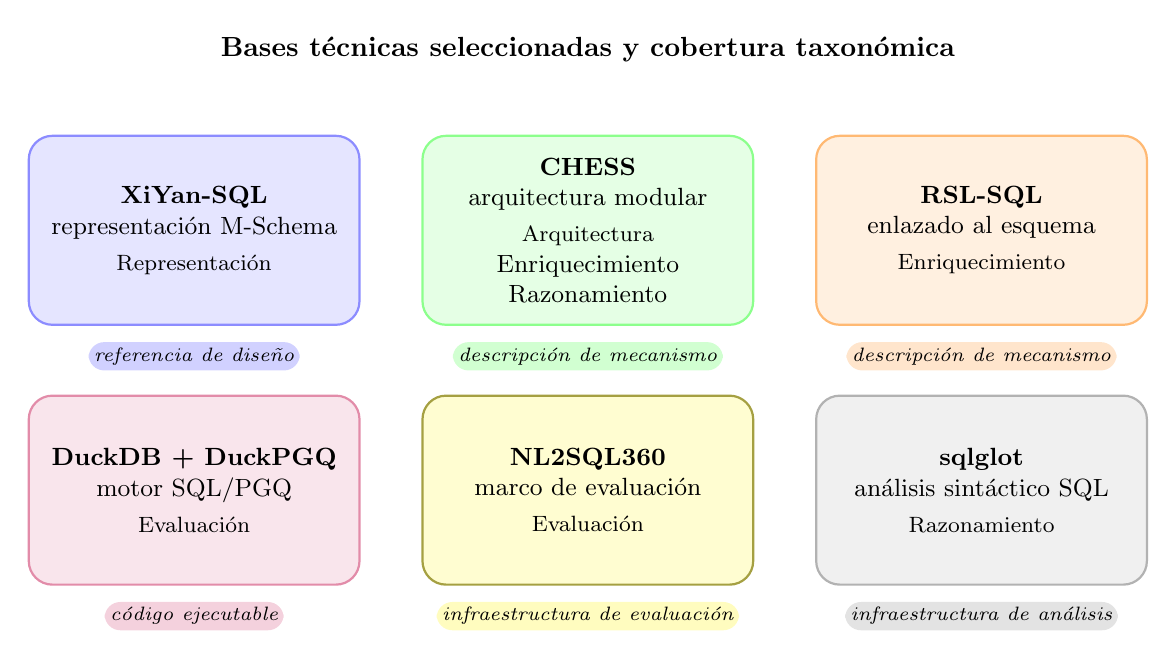
\begin{tikzpicture}[
    font=\small,
    base/.style={
        rectangle,
        rounded corners=3mm,
        draw,
        thick,
        align=center,
        minimum width=4.2cm,
        minimum height=2.4cm,
        inner sep=5pt
    },
    role/.style={
        font=\scriptsize\itshape,
        rounded corners=2mm,
        inner sep=2pt
    }
]

\node[font=\bfseries] at (5,2.3)
    {Bases técnicas seleccionadas y cobertura taxonómica};

\node[base, fill=blue!10, draw=blue!45] at (0,0) {
    \textbf{XiYan-SQL}\\
    representación M-Schema\\[2pt]
    \footnotesize Representación
};

\node[base, fill=green!10, draw=green!45] at (5,0) {
    \textbf{CHESS}\\
    arquitectura modular\\[2pt]
    \footnotesize Arquitectura\\
    Enriquecimiento\\
    Razonamiento
};

\node[base, fill=orange!12, draw=orange!55] at (10,0) {
    \textbf{RSL-SQL}\\
    enlazado al esquema\\[2pt]
    \footnotesize Enriquecimiento
};

\node[base, fill=purple!10, draw=purple!45] at (0,-3.3) {
    \textbf{DuckDB + DuckPGQ}\\
    motor SQL/PGQ\\[2pt]
    \footnotesize Evaluación
};

\node[base, fill=yellow!18, draw=yellow!60!black] at (5,-3.3) {
    \textbf{NL2SQL360}\\
    marco de evaluación\\[2pt]
    \footnotesize Evaluación
};

\node[base, fill=gray!12, draw=gray!60] at (10,-3.3) {
    \textbf{sqlglot}\\
    análisis sintáctico SQL\\[2pt]
    \footnotesize Razonamiento
};

\node[role, fill=blue!18] at (0,-1.6) {referencia de diseño};
\node[role, fill=green!18] at (5,-1.6) {descripción de mecanismo};
\node[role, fill=orange!20] at (10,-1.6) {descripción de mecanismo};

\node[role, fill=purple!18] at (0,-4.9) {código ejecutable};
\node[role, fill=yellow!25] at (5,-4.9) {infraestructura de evaluación};
\node[role, fill=gray!22] at (10,-4.9) {infraestructura de análisis};

\end{tikzpicture}
